%%%%%%%%%%%%%%%%%%%%%%%%%%%%%%%%%%%%%%%%%
% Stylish Article
% LaTeX Template
% Version 1.0 (31/1/13)
%
% This template has been downloaded from:
% http://www.LaTeXTemplates.com
%
% Original author:
% Mathias Legrand (legrand.mathias@gmail.com)
%
% License:
% CC BY-NC-SA 3.0 (http://creativecommons.org/licenses/by-nc-sa/3.0/)
%
%%%%%%%%%%%%%%%%%%%%%%%%%%%%%%%%%%%%%%%%%

%----------------------------------------------------------------------------------------
%	PACKAGES AND OTHER DOCUMENT CONFIGURATIONS
%----------------------------------------------------------------------------------------

\documentclass[fleqn,10pt,ngerman]{SelfArx}

\usepackage{babel}
\selectlanguage{ngerman}

\setlength{\columnsep}{0.55cm} % Distance between the two columns of text
\setlength{\fboxrule}{0.75pt} % Width of the border around the abstract

\definecolor{color1}{RGB}{0,0,90} % Color of the article title and sections
\definecolor{color2}{RGB}{0,20,20} % Color of the boxes behind the abstract and headings

\newlength{\tocsep} 
\setlength\tocsep{1.5pc} % Sets the indentation of the sections in the table of contents
\setcounter{tocdepth}{2} % Show only three levels in the table of contents section: sections, subsections and subsubsections


\usepackage{fontenc}
\usepackage{inputenc}
\usepackage{url} 


%----------------------------------------------------------------------------------------
%	ARTICLE INFORMATION
%----------------------------------------------------------------------------------------

\JournalInfo{Praxisbericht} % Journal information
\Archive{Wintersemester 16/17} % Additional notes (e.g. copyright, DOI, review/research article)

\PaperTitle{REST Anwendungsarchitektur} % Article title

\Authors{Max Mustermann} % Authors
\affiliation{\textit{Hochschule Kaiserslautern}} % Author affiliation
\affiliation{\textbf{Corresponding author}: max.mustermann@fh-kl.de} % Corresponding author

\Keywords{Web-Entwicklung, RESTful, SOA, JSON, Design, Java} % Keywords - if you don't want any simply remove all the text between the curly brackets
\newcommand{\keywordname}{Keywords} % Defines the keywords heading name

%----------------------------------------------------------------------------------------
%	ABSTRACT
%----------------------------------------------------------------------------------------

\Abstract{Das Abstract ist eine maximal 200 Worte lange Zusammenfassung des Inhalts der Arbeit, so dass sich der Leser vorab ein erstes Bild vom Inhalt machen kann.}

%----------------------------------------------------------------------------------------

\begin{document}

\flushbottom % Makes all text pages the same height

\maketitle % Print the title and abstract box

\tableofcontents % Print the contents section

\thispagestyle{empty} % Removes page numbering from the first page

%----------------------------------------------------------------------------------------
%	ARTICLE CONTENTS
%----------------------------------------------------------------------------------------

\section*{Einleitung} % The \section*{} command stops section numbering

\addcontentsline{toc}{section}{\hspace*{-\tocsep}Einleitung} % Adds this section to the table of contents with negative horizontal space equal to the indent for the numbered sections

Die Einleitung sollte ausreichenden Hintergrund für den Leser liefern, so dass er sich ohne großes Studium von Sekundärliteratur
in das Thema hineindenken kann. Auch sollte die Aufgabenstellung bzw. Motivation für die vorliegende Arbeit dargelegt werden, sowie die Zielsetzung, die man erreichen will. Weiter wird auch das Thema von eventuell verwandten Themen abgegrenzt. Hier kann auch die Literatur \cite{Harel:1987,Harel2006} und \cite{Gurp99onthe} vorgestellt werden.

Konkret sollt hier das Ziel und die Motivation des Projekts erläutert werden. Am Ende des Abschnitts steht eine kurze Übersicht über die weiteren Abschnitte.

Auch wenn die Einleitung zu Beginn der Arbeit liegt, wird sie oft erst am Ende verfasst.

%------------------------------------------------

\section{REST: State of the art}
Um zu verstehen, weshalb REST allgegenwärtig in der Entwicklung von Web-Applikationen ist, werden im Folgenden die Eigenschaften datiert, welche ein REST Interface spezifiziert. Um weiterhin die Unterschiede, sowie Vor- und Nachteile, zu diskutieren, wird eine Gegenüberstellung mit dem SOAP (\textit{Simple Object Access Protocol}) vorgenommen. 

\subsection{Paradigmen und Eigenschaften}
Die Aufbau aktueller Web-Applikationen beruht auf der Überlegung einer Service orientierten Kommunikation. Aufbauend auf der \textit{Service Oriented Aarchitecture(SOA)} wurde vom W3C die Definition für die noch heute gültige \textit{Web Services Architecture}(vgl. \cite{WSA}) festgelegt. Hier wird schon REST als Modell für das konstruieren für Web Services verwendet. Eine schematische Veranschaulichung finde sich Abbildung \ref{fig:rest}. Um jedoch eine REST-konforme Architektur zu realisieren wurden von Roy Thomas Fielding in seiner Dissertation\cite{Fielding:2000} eine Anzahl von Voraussetzungen festgeschrieben, die eine Architektur auf Basis von REST erfüllen muss:
\begin{figure}[ht]\centering
	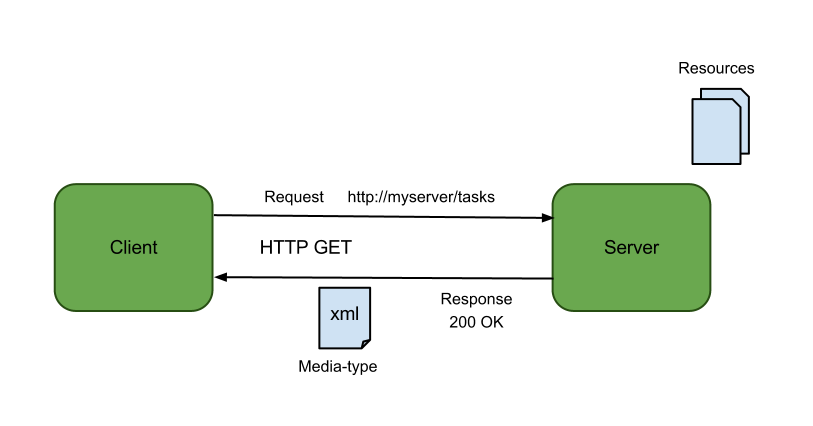
\includegraphics[width=9 cm]{Abbildungen/REST.png}
	\caption{Schematischer Aufbau WSA via REST. Quelle: http://www.prideparrot.com/}
	\label{fig:rest}
\end{figure}

\begin{itemize}
	\item \textbf{Client-Server:}\\ Der Ansatz der Client-Server Architektur soll verfolgt werden. Durch das Lösen der UI von den Daten der Applikation wird eine Portabilität, Skalierbarkeit und das Vereinfachen der Server-Komponente realisiert, was mittlerweile als Grundlage der kompletten Internet-Architektur gilt, denn der HTTP-Standard selbst beruht auf dieser Architektur.
	\item \textbf{Stateless:}\\ Die Zustandslosigkeit gilt für die Kommunikation zwischen Client und Server. Anfragen des Clients müssen alle Information enthalten um vom Server identifiziert und bearbeitet werden zu können. Einen Zustand oder Session-Informationen liegen somit komplett auf Seiten des Clients.
	\item \textbf{Cache:}\\ Die Antwort auf eine Client-Anfrage kann vom Server als cacheble oder non-cacheble gelabelt werden. Der Cache befindet sich auf der Client-Seite und erlaubt dem Client die Antwort für weitere Anfragen gleicher Art zu verwenden. Dadurch kann teilweise eine Kommunikation zwischen Client und Server unterbunden werden was die Performanz und Effizienz client-seitig stark erhöhen kann.
	\item \textbf{Uniform Interface:}\\ Das Uniform Interface repräsentiert das fundamentale Wesen eines REST-Services. Durch die Uniformierung jeder Ressource werden die Daten von der Architektur gelöst, was eine starke Entkopplung sowie Vereinfachung der Interaktion mit sich bringt. Weiterhin soll jeder Client die nötigen Information und Daten erhalten, die es ihm erlaubt, Ressourcen zu identifizieren und dadurch auch zu modifizieren. Die angefragte Ressource muss nicht die selbe Repräsentation auf Server- und Client-Seite besitzen. Objekte vom Server werden also zum Beispiel via XML oder JSON übertragen, enthalten die definierten Daten, müssen aber nicht dem Datentyp des Server-Objekts entsprechen. Nach Fieldings ist hier das \textit{Hypermedia as the engine of application state (HATEOAS)}-Prinzip mit der wichtigste Faktor. Dieses besagt, dass der Client alle Ressourcen nur über die definierten URI's beziehen kann. Durch diesen Zugang kann der Server dynamisch Daten kommunizieren und weiter verfügbare Adressen der Antwort hinzufügen. Somit wird verhindert, dass der Client fest codierte Information enthalten muss. Dadurch entsteht die Flexibilität des REST-Services.
	\item \textbf{Layered System:}\\ Dem Client muss nicht bekannt sein, ob die Kommunikation direkt mit dem Server stattfindet oder nicht. Die Anfrage wird gestellt und welcher Server aus einem Kollektiv die Antwort sendet, kann nicht zugeordnet werden. Dadurch können Prinzipien wie Load-Balancing und unterschiedliche Web-Sicherheitskriterien realisiert werden. 
	\item \textbf{Code on demand(optional):}\\ Dieser Schritt ist optional und beschreibt die Möglichkeit nach Anfrage ausführbaren Code vom Server zum Client zu transferieren, wie zum Beispiel Skripte in JavaScript. Somit kann der Server zeitweise die Funktionalität der Client-Applikation beeinflussen.
\end{itemize} 

\begin{figure}[ht]\centering
	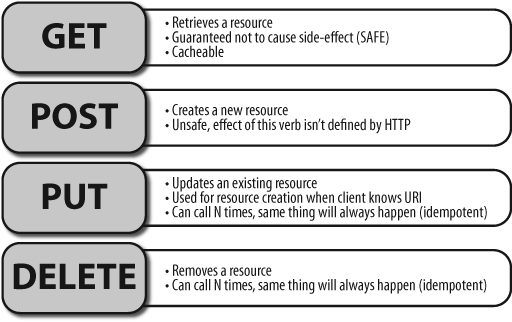
\includegraphics[width=8.5 cm]{Abbildungen/RESTful-operations}
	\caption{Beschreibung der Standard HTTP Methoden in der REST-Architektur. Quelle: http://www.itersdesktop.com/}
	\label{fig:restCalls}
\end{figure}

Im Kontext von Web-Services, welche sich an die REST-Vorgaben binden, wird zumeist die Kommunikation über HTTP umgesetzt. Die API wird über eine Basis-URL angesprochen, über welche dann die benötigten Ressourcen angefragt werden müssen. HTTP bietet eine gewisse Anzahl an Standardmethoden(hauptsächlich: \textit{GET, PUT, POST, DELETE}) die auch für den Datentransfer in einer RESTful-API genutzt werden. Die grundlegenden Eigenschafen der Methoden finden sich im Bild \ref{fig:restCalls}. Diese Methoden repräsentieren auch die bekannten \textit{CRUD}-Operationen(Create, Read, Update, Delete) zur Datenverwaltung und Datenverarbeitung. Eine mögliche Variante mit den entsprechenden HTTP-Befehlen ist in der Tabelle \ref{tab:httptable} zu sehen. Es gilt weiterhin zu erwähnen, dass eine URL mit der entsprechenden HTTP-Methode als eindeutig gilt. Die URL kann jedoch mit einer weiteren HTTP-Methode genutzt werden. Dadurch wird festgelegt welche von den CRUD-Operation auf die entsprechende Ressource angewandt werden darf. 

\begin{table}[hbt]
	\caption{HTTP Methoden für spezifische URL's}
	\centering
	\begin{tabular}{ |p{2cm}|p{5.5cm}|}
		\toprule
		\cmidrule(r){1-2}
		URL & \textbf{http://api.example.com/res/item42}\\
		\midrule
		GET & Eine Repräsentation des Items42 wird an den Client übertragen\\
		\midrule
		POST & Wird zum Erstellen neuer Ressourcen verwendet, würde in diesem Fall eher nicht genutzt werden\\
		\midrule
		PUT & Item42 wird überschrieben oder erstellt wenn noch nicht vorhanden\\
		\midrule
		DELETE & Das adressierte Element Item42 wird gelöscht\\
		\bottomrule
	\end{tabular}\\
	\label{tab:httptable}
\end{table}

\subsection{REST vs. SOAP}
Bevor sich REST im Bereich der verteilten Anwendung etablierte war die größte Vertreter für die Kommunikation innerhalb einer SOA das SOAP. Bei SOAP handelt es sich um eine RPC Middleware die HTTP oder SMTP als Transportprotokoll für XML als Nachrichtenformat verwendet. Schon im grundsätzlichen Ansatz unterscheiden sich beide Herangehensweisen. Wird bei REST von einer exakten Uniformierung jeder Ressource gesprochen, die somit auch immer separat angesprochen werden können, so wird bei SOAP mit einem Dispacher gearbeitet. In sogenannten Envelopes werden alle Anfragen an den Server via XML mit dem HTTP-Post-Befehl an den zentralen Dispatcher geleitet. Die Anfrage gehen an genau eine URL die den Dispatcher adressiert. Im Listing \ref{envelopesoap} ist ein SOAP-Request mit seiner korrespondierenden Response zu sehen. Im Body wird eine \textit{GetStockPrice} Anfrage gestellt für das Unternehmen IBM. Im Body der Antwort wird somit die \textit{GetStockPriceResponse} mit dem Wert von 34,5 übermittelt. Die URL \textit{http://www.example.org/stock} spricht den Dispatcher des Webservers an. Dieser verteilt die Anfrage an die richtige Methode, hier \textit{GetStockPrice}. Diese Methode muss auf dem Server verfügbar sein. Durch die Anfrage wird ein Methodenaufruf mit den gelieferten Parametern durchgeführt. Das Ergebnis des Methodenaufrufs wird als Response in einem neuen Envelope zurück geliefert. Da jede Antwort einer exakten Anfrage gilt, ist ein erneutes stellen der gleichen Anfrage nicht möglich. Somit entfällt eine Möglichkeit caching auf Seiten des Clients zu betreiben.

\begin{lstlisting}[caption=Beispiel: SOAP-Request und SOAP-Response als Envelope, label=envelopesoap]
 POST /InStock HTTP/1.1
Host: www.example.org
Content-Type: application/soap+xml; charset=utf-8
Content-Length: nnn

<?xml version="1.0"?>

<soap:Envelope
xmlns:soap="http://www.w3.org/2003/05/soap-envelope/"
soap:encodingStyle="http://www.w3.org/2003/05/soap-encoding">

<soap:Body xmlns:m="http://www.example.org/stock">
<m:GetStockPrice>
<m:StockName>IBM</m:StockName>
</m:GetStockPrice>
</soap:Body>

</soap:Envelope>

--------------------------------------------

 HTTP/1.1 200 OK
Content-Type: application/soap+xml; charset=utf-8
Content-Length: nnn

<?xml version="1.0"?>

<soap:Envelope
xmlns:soap="http://www.w3.org/2003/05/soap-envelope/"
soap:encodingStyle="http://www.w3.org/2003/05/soap-encoding">

<soap:Body xmlns:m="http://www.example.org/stock">
<m:GetStockPriceResponse>
<m:Price>34.5</m:Price>
</m:GetStockPriceResponse>
</soap:Body>

</soap:Envelope>
\end{lstlisting}
Ebenso wie REST wurde SOAP vom W3C spezifiziert. Unterschied ist allerdings, bei REST handelt sich um einen Architekturstil bei SOAP um ein Protokoll. in der Spezifikation steht zum Beispiel, dass ausschließlich XML als Datenformat verwendet wird und was ein XML wohl definiert um als SOAP konform zu gelten(\cite{w3cSOAP}). Der Unterschied zu REST liegt hier darin, dass außer XML bei REST weitere Datenformate wie zum Beispiel JSON und YAML verwendet werden können. Die genaue Adressierung der Ressourcen unter REST erlaubt eine leichtgewichtige Transportmöglichkeit. Metadaten, wie das Encoding oder der Content-Type, werden im Header des HTTP-Requests codiert. Zusätzliche Information werden nicht benötigt. SOAP hingegen bietet diese Möglichkeit nicht. Durch die Konvention, welche Bestandteile ein XML-Envelope vorzuweisen hat, ist diese Leichtigkeit nicht zu erreichen. Das XML-Dokument muss auf Seiten des Sender aufgebaut und anschließen validiert werden um die Konformität zu bewahren. Dadurch werden zusätzliche Metadaten zur Beschreibung der Datei dem XML-Dokument hinzugefügt. Gerade bei einfachen Anfrage, zum Beispiel eine Zustandsabfrage wahr oder falsch, ist das Verhältnis von Nutz- zu Metadaten eher mäßig. Je aufwändiger die Anfrage desto besser entwickelt sich das Nutzlastenverhältnis. Anfragen eine XML-Dokuments werden immer atomar ausgeführt. Somit können komplexe Sachverhalte in einer Anfrage definiert werden und sequentiell abgearbeitet werden. Bei REST werden meist leichtgewichtige Schnittstellen exponiert die genau eine Anfrage nach einer bestimmten Ressource beantworten. Somit sind bei komplexeren Schritten mehre Anfragen nötig. Dadurch ist der Kommunikationsaufwand etwas höher als bei SOAP. Relativ ähnlich verhalten sich die beiden in Bezug auf die Interaktion. Da beide Plattform unabhängige Datenformate verwenden entfaltet sich ein großen Potenzial in der Nutzung. Programme jeglicher Art, entwickelt in einer belieben Programmiersprache, welche die Datenformate ebenso unterstützen, können mit den Schnittstellen interagieren. Bei REST muss eine API-Beschreibung mit den exponierten URL's, bei SOAP die URL mit den möglichen Methodenaufrufen öffentlich gemacht werden. Bei SOAP wird die Beschreibung meist als WSDL(\textit{Web Services Description Language})(vgl. \cite{w3cWSDL}) vorgelegt. In dem WSDL-File werden alle Funktionen, Daten und Datentypen beschrieben. Es werden im wesentlichen die Operation definiert, die von außen zugänglich sind. Mit diesem WSDL-File wird auch die Validierung des XML-Dokuments durchgeführt. Es handelt sich auch hierbei um einen weiteren Standard definiert vom W3C.
\subsection{Evaluierung}
Durch die Kriterien welche Fieldings vorgibt, sowie durch den Vergleich mit SOAP haben sich einige Punkte heraus kristallisiert, welche hier nochmals kurz zusammen gefasst werden. \\ REST wird als leichte Schnittstelle definiert, in welcher jede URL eine exakte Ressource anspricht. Die Kommunikation findet über HTTP mit den üblichen HTTP-Methoden statt. Dem Client ist nicht bekannt man wem oder was die Kommunikation stattfindet was eine hohe Flexibilität und Skalierbarkeit generiert. Es müssen für alle benötigten Information immer die entsprechenden Requests angefragt werden, was wiederum zu einer starken Kommunikation mit Client und Server führt. Durch caching auf der Client-Seite kann dem etwas vorgebeugt werden. Meta-Informationen werden innerhalb des HTTP-Headers gespeichert und im Body befinden sich nur die Nutzdaten. Dadurch wird ein guten Nutzlastenverhältnis produziert. Die Information des Bodys kann in unterschiedlichen Datenformaten verschickt werden, was eine vielfältige Anwendungsmöglichkeit bietet. \\ Durch die vielen Vorteile ist leicht nachzuvollziehen wieso REST aktuell der vorherrschende Architektur Stil in Sachen Web-Anwendung ist. Im Bereich von großen Enterprise-Lösungen bis hin zu kleinen leichten Web-Anwendung zur Kommunikation mit einer mobilen Applikation werden mit REST realisiert. 

\section{Entwicklungsansatz und Aufbau}
Kurze Einführung in den Abschnitt. Es wird beschrieben was jetzt kommt. Erklärung Beispiel Projekt

\subsection{JAX-RS - die Basis für REST-Services in JAVA}
Erläuterung der API, Bestandteile, Features 

\subsection{Serverseite Beispielimplementierung}
Erläuterung der API, Bestandteile, Features 

\subsection{Clientseite Beispielimplementierung}
Erläuterung der API, Bestandteile, Features 

\section{Frameworks? Microservice-Architektur?}

\section{Zusammenfassung}
Hier wird nochmal der Inhalt und die Ergebnisse der Arbeit erörtert. Im Ausblick werden Themen und Aufgabenstellungen genannt, die es lohnt weiter zu untersuchen.

%----------------------------------------------------------------------------------------
%	REFERENCE LIST
%----------------------------------------------------------------------------------------

\bibliographystyle{unsrt}
\bibliography{Literatur}

%----------------------------------------------------------------------------------------

\subsubsection*{Erklärung zur Ausarbeitung}
Hiermit erkläre ich, {\it Vorname Nachname (Matrikel)}, dass ich die vorliegende Ausarbeitung selbstständig und ohne fremde Hilfe angefertigt habe und keine anderen als in der Abhandlung angegebenen Hilfen benutzt habe; dass ich die Übernahme wörtlicher Zitate aus der Literatur sowie die Verwendung der Gedanken anderer Autoren an den entsprechenden Stellen innerhalb der Arbeit gekennzeichnet habe. Ich bin mir bewusst, dass eine falsche Erklärung rechtliche Folgen haben kann.\\ \\
--------------------- \\
Unterschrift


\clearpage
\newpage
\appendix
\section{Bemerkungen zur Ausarbeitung}
Der Umfang der Ausarbeitung sollte 10 Seiten nicht übersteigen. Die Ausarbeitung sollte dem Charakter nach eher einem {\it scientific paper} entsprechen. Siehe hierzu auch  \cite{Rechenberg}. Keine Ich-Form benutzen. Aussagen sollten möglichst belegt oder begründet werden.

Die schriftliche Ausarbeitung hat folgende Zwecke:
\begin{itemize}[noitemsep]
\item die Ausarbeitung soll Kommilitonen (die nicht an der Veranstaltung teilgenommen haben) in das Thema ein\-führen.
\item die Autorin bzw. der Autor soll üben, wie man technische Sachverhalte kurz und klar beschriebt.
\item die Ausarbeitung bildet die Grundlage der Bewertung. In der Arbeit soll
gezeigt werden, dass man das Thema geistig durchdrungen hat.
\end{itemize}


\subsection{Latex-Syntax}
Im folgenden finden Sie einige nützliche Latex-Anweisungen.

Abbildung \ref{fig:MultiInterfaces} zeigt ein Bild, dass die komplette Seitenbreite einnimmt. Abbildung \ref{fig:Baustein} ist dagegen in die Spalte eingebettet.


\begin{figure}[ht]\centering
	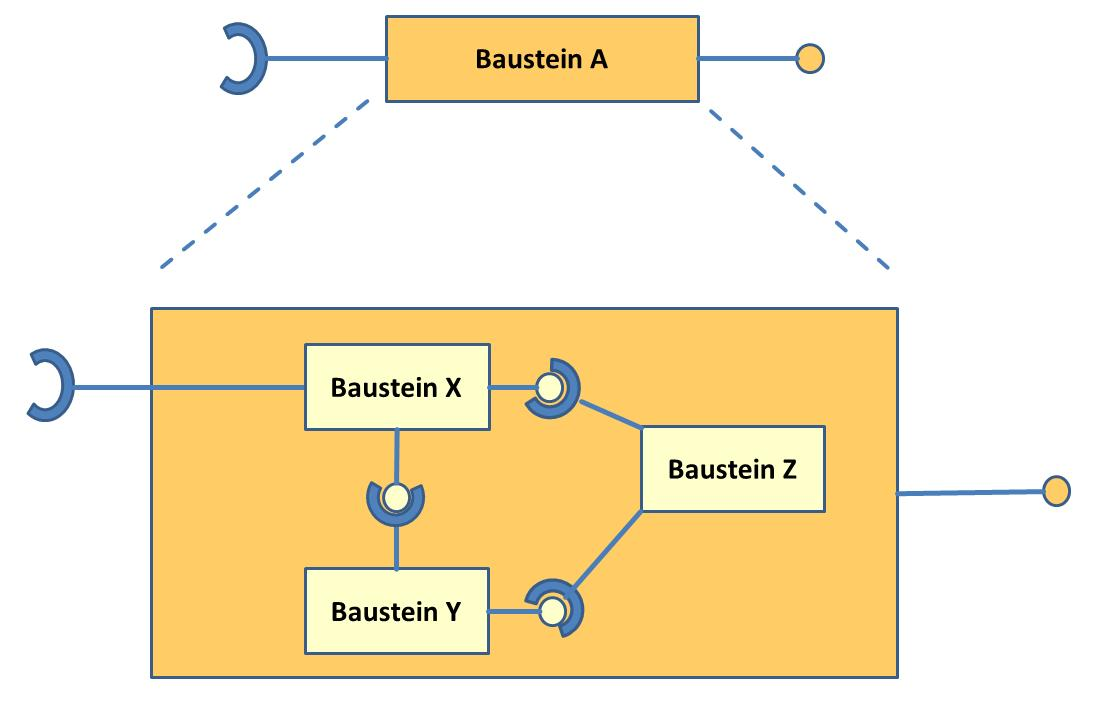
\includegraphics[width=5 cm]{Abbildungen/Baustein}
	\caption{Beispiel für ein Bild in der Spalte}
	\label{fig:Baustein}
\end{figure}

\begin{figure*}[ht]\centering % Using \begin{figure*} makes the figure take up the entire width of the page
	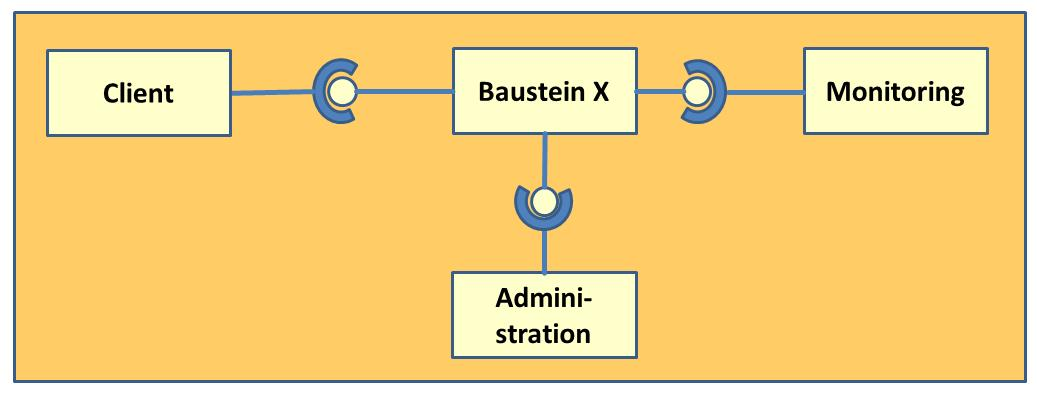
\includegraphics[width=\linewidth]{Abbildungen/BausteinMultiInterfaces}
	\caption{Beispiel für ein breites Bild}
	\label{fig:MultiInterfaces}
\end{figure*}

Hier sehen Sie, wie man ein Java-Code-Listing mit einbinden kann. Es kann auch ein Label vergeben werden, auf das dann referenziert werden kann (vgl. Listing \ref{Test}). 
\begin{lstlisting}[caption=Eine Testklasse, label=Test]
public class Test
{
  private int mCount = 0;
	
  @Override	
  public void xyz()
  {
    for(int i = 0; i< 10; i++)
    {
      this.mCount += i;
    }
	
    // Ein Kommentar		
    this.mEnd = this.mCount;
  }
}
\end{lstlisting}


Hier ein Beispiel für eine mathematische Formel ohne Nummer
\begin{equation*}
	\cos^3 \theta =\frac{1}{4}\cos\theta+\frac{3}{4}\cos 3\theta
	\label{eq:refname2}
\end{equation*}

Oder mehrere mathematische Ausdrücke untereinander
\begin{eqnarray}
	f(x) &=& \frac{3 e^x}{1 - x^2} \\
	g(x) &=& \sqrt[3]{\sin \alpha} \\
	h(x) &=& \frac{2 + 3i}{1- i}
\end{eqnarray}

Hier noch ein Beispiel für eine Aufzählung, wobei die Aufzählungspunkte direkt nacheinander, d.h. ohne Leerzeile, aufgelistet werden.
\begin{enumerate}[noitemsep] % [noitemsep] removes whitespace between the items for a compact look
	\item First item in a list
	\item Second item in a list
	\item Third item in a list
\end{enumerate}

Ein Beispiel für eine Tabelle, falls man ein solches Konstrukt benötigt.

\begin{table}[hbt]
	\caption{Table of Grades}
	\centering
	\begin{tabular}{llr}
		\toprule
		\multicolumn{2}{c}{Name} \\
		\cmidrule(r){1-2}
		First name & Last Name & Grade \\
		\midrule
		John & Doe & $7.5$ \\
		Richard & Miles & $2$ \\
		\bottomrule
	\end{tabular}
	\label{tab:label}
\end{table}

Siehe Tabelle \ref{tab:label}.
Und hier nochmal das Einbinden eines Bildes (vgl. Abb. \ref{fig:Schnittstellen}.), wobei das Bild innerhalb der Spalte gezeigt wird.


\begin{figure}[ht]\centering
	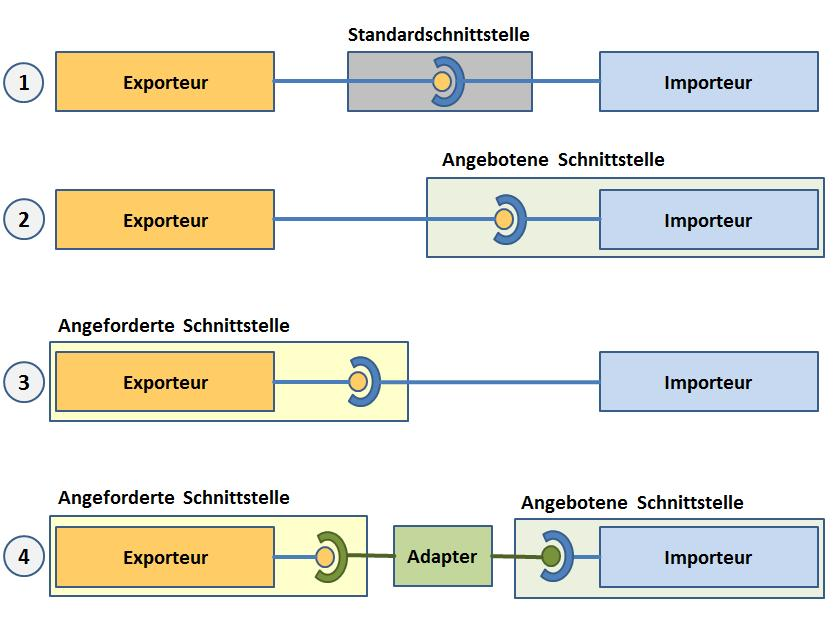
\includegraphics[width=5 cm]{Abbildungen/Schnittstellen}
	\caption{Beispiel für ein Bild in der Spalte}
	\label{fig:Schnittstellen}
\end{figure}

\subsection{Allgemeine Hinweise}
Bei den Ausführungen fasst man sich so kurz wie möglich, aber so lange wie nötig um verständlich zu sein. Man schreibt die Projektarbeit für Leser, die die gleichen Vorkenntnisse haben wie man selbst.
Die Projektarbeit besitzt im Prinzip den selben Aufbau wie dieses Dokument.

Eine Arbeit wird nur einmal geschrieben aber von vielen, d.h. oft gelesen. Der Verfasser sollte es sich deshalb bei der Formulierung schwer machen, damit es der Leser später um so leichter hat. Benutzen Sie Bilder und legen Sie einen roten Faden durch Ihren Text.

\subsection{Bemerkungen zur Literatur}
Die Literaturliste muss die Referenzen enthalten, auf die man vorher verwiesen hat - nicht mehr und nicht weniger. Sie werden sicherlich sehr oft referenzieren. Wenn ein Artikel eine Web-Adresse hat, muss die Web-Adresse aufgenommen werden, vgl. \cite{RobertMartinOOMetrics} oder \cite{RobertMartinSOLID}.




%------------------------------------------------


\section{Formalien}
\subsection{Bewertungskriterien}
Damit die Arbeit nicht nur eine reine Zusammenfassung des Vorlesungsinhalts bleibt, soll die Projektarbeit auch einen {\it Eigenanteil} enthalten. Dieser Eigenanteil kann z.B. eine eigene Literaturrecherche sein und somit Themen aufgreifen, die nicht explizit in der Veranstaltung besprochen wurden.


In die Bewertung der Projektarbeit gehen folgende Punkte mit ein:
\begin{enumerate}[noitemsep]
\item Formale Kriterien: Äußere Form, Layout, Zitiertechnik und korrekte Angabe der Literatur, Stil, Abbildungen, Rechtschreibung, etc.
\item Systematik der Darstellung: Vollständigkeit (Wie breit und tiefgehend wird das Thema behandelt?), korrekte Wiedergabe (wurde das Thema richtig verstanden), logische Gliederung und Gedankenführung
\item Eigenständigkeit der Darstellung: Wurde in eigenen Worten zusammengefasst oder nur Zitate benutzt? Präsen\-tation des Themas (Didaktik), wurden Aussagen zueinander in Beziehung gesetzt und wurde ein eigener gedanklicher Aufbau gewählt?
\item Tiefe und Umfang des Eigenanteils: Hat der Eigenanteil fachliche Substanz? Innovationspotential, d.h. wie viele eigene Ideen wurden eingebracht.
\end{enumerate}


\cleardoublepage
\newpage
\onecolumn

\section{Listings}
Hier im Anhang sind Listings aufgeführt, die besser im ,,großen'' einspaltigen Format wiedergegeben werden. 

\begin{lstlisting}[caption=Der Levenshtein Algorithmus, label=Lst:LevenshteinAlgorithm]

import spellchecker.algorithm.EditDistance;

public class LevenshteinAlgorithm implements EditDistance
{
  public final int distance(String from, String to)
  {
     assert from != null && to != null : "Parameters should not be null";

     // Sonderfaelle
     if (from.equals(to))    return 0;
     if (from.length() == 0) return to.length();
     if (to.length() == 0)   return from.length();

     int width = from.length() + 1;
     int height = to.length() + 1;

     // Tabelle
     int[][] table = new int[height][width];

     // Initialisierung erste Zeile
     for (int i = 0; i < width; i++)
     {
        table[0][i] = i;
     }

     // Zeilen (to)
     for (int i = 1; i < height; i++)
     {
        table[i][0] = i;
        // Spalten (from)
        for (int j = 1; j < width; j++)
        {
           int delta = 0;
           if (to.charAt(i - 1) != from.charAt(j - 1))
               delta = 1;

           table[i][j] = min( 
                table[i][j-1] + 1, table[i-1][j] + 1, table[i-1][j-1] + delta );
        }
     }

     return table[height-1][width-1];
  }

  public final static int min(int a, int b, int c)
  {
     if (a < b && a < c)
         return a;
     else if (b < c)
        return b;
     else
       return c;
   }
}
\end{lstlisting}


\end{document}